\documentclass[10pt]{article}

\addtolength{\oddsidemargin}{-.875in}
\addtolength{\evensidemargin}{-.875in}
\addtolength{\textwidth}{1.75in}

\addtolength{\topmargin}{-.875in}
\addtolength{\textheight}{1.75in}

\openup 1em

%macro for commenting
\usepackage{color}
\newcommand{\leo}[1]{{\color{blue}{\it leo: #1}}}

% \newcommand{\Xbeta}{ X_i \theta}
\newcommand{\xbeta}{ x_i \beta}
\newcommand{\xtheta}{ x_i \theta}
% \newcommand{\xbetaij}{ x_{ij}^T \theta}
\newcommand{\sgamma}{s_{ij}^T\gamma_i}

\usepackage[round]{natbib}

\usepackage{rotating}
\usepackage{graphicx}
\usepackage{subcaption}

\usepackage{float}
\usepackage{bbm}

\usepackage{amsthm,amsmath} 
\usepackage{amssymb}
\usepackage{mathrsfs}
\usepackage{subcaption}
\usepackage{nicefrac}

\newtheorem{theorem}{Theorem}
\newtheorem{lemma}{Lemma}
\newtheorem{corollary}{Corollary}
\newtheorem{remark}{Remark}


\usepackage{algorithm}
\usepackage{algpseudocode}

%\usepackage{mhequ}
\newcommand{\be}{\begin{equation}\begin{aligned}}
\newcommand{\ee}{\end{aligned}\end{equation}}
\newcommand{\bb}[1]{\mathbb{#1}}
\newcommand{\mc}[1]{\mathcal{#1}}
\DeclareMathOperator{\Binom}{Binomial}
\DeclareMathOperator{\No}{No}
\DeclareMathOperator{\PG}{PG}
\DeclareMathOperator{\IG}{Inverse-Gamma}
\DeclareMathOperator{\Ga}{Gamma}
\DeclareMathOperator{\Bern}{Bernoulli}
\DeclareMathOperator{\U}{Uniform}
\DeclareMathOperator{\Poi}{Poisson}
\DeclareMathOperator{\NB}{NB}
\DeclareMathOperator{\cov}{cov}
\DeclareMathOperator{\var}{var}
\DeclareMathOperator{\diag}{diag}
\DeclareMathOperator{\Diag}{Diag}
\newcommand{\KL}[2]{\textnormal{KL}\left(#1 \parallel #2\right)}

\DeclareMathOperator{\bigO}{\mc O}



\thispagestyle{empty}
\baselineskip=28pt

\title{\textbf{Extrinsic Prior for Simple and Efficient\\ Bayesian Modeling with Parameter Constraints}}
%\author{Leo Duan, David Dunson}
\date{}
\begin{document}

\maketitle


{\bf Abstract:} Parameter constraints are very common in statistical models. Examples include linear inequality, parameter ordering, monotonicity, orthogonality, etc. Bayesian approach is useful for uncerntainty quantification in the constrained space. Although specific solutions have been made for different constraints, it is challenging to incorporate them in advanced applications, such as modeling with non-parametric assumption or high-dimensional data. In this paper, we propose a simple and general solution by first replacing constraints with strongly informative prior. Through this {\it extrinsic} prior, the parameters are relaxed to a less restrictive space, where conventional tools such as Hamiltonian Monte Carlo are utilized to obtain approximate posterior. Then these posteriors can be easily projected back to the constrained space for exact solution. This approach is very efficient and applicable to a wide range of problems with equality and inequality constraints. The generality allows more families of prior to be chosen for the constrained parameters, and simplifies the adoption of multiple constraints for desired property such as identifiability. Theory is developed and novel statistical applications under constraints are illustrated.
\vskip 12pt

%\baselineskip=12pt
%\par\vfill\noindent
{\noindent  KEY WORDS:  Constraint violation; Space embedding; Monotone Dirichlet; Orthogonal Gaussian processes; Posterior mixing; Projected Markov chain}
%\par\medskip\noindent
%\clearpage\pagebreak\newpage
\pagenumbering{arabic}

\section{Introduction}

Constraints are very common in modern statistical modeling. For example, functional data anaylsis often impose certain shape constraint such as monotonicity or convexity on curves \citep{kelly1990monotone}; matrix and tensor decomposition utilize orthonormality for better identifiability \citep{uschmajew2010well}; many manifolds such as simplex can be considered as sub-manifolds of a Euclidean space embedded via certain constraints.

Constraints can cause substantial modeling difficulty. When data are in constrained space, parameters can enter the likelihood via an integral without closed-form, commonly known as ``doubly intractable'' problem. Successful solutions have been proposed to address this issue \citep{murray2012mcmc,rao2016data}. When parameters are in  constrained space, challenges often arise in the difficulty for estimation under constraint. Frequentist optimization literature often relies on Lagrange and Karush-Kuhn-Tucker multipliers for point estimate under equality and inequality constraints \citep{boyd2004convex}. However, the uncertainty quantification is difficult since conventional asympotic result on variance estimation often no longer hold in constrained space. Bayesian approach is more approriate for this purpose.

There have been a wide range of solutions developed for specific constraints. One strategy involves using constrained prior with posterior that can be conveniently sampled. For example, to model othornormal matrices on the Stiefel manifold, Bingham-von-Mises-Fisher distribution \citep{khatri1977mises,hoff2009simulation} is a parametric family with a closed-form posterior in matrix and tensor decomposition. \cite{lin2016bayesstiefel} extends the flexibility of matrix von-Mises-Fisher distribution via non-parametric approach. Another strategy is to bypass the constraint via re-parameterization. The famous example is the stick-breaking construction for Dirichlet distribution and process. The re-parameterization essentially utilizes the coordinate system of the simplex, and circumvents the norm constraint on the probability vertices. As these methods directly satisfy the constraint requirement, we refer them as the intrinsic approaches. Despite the success of intrinsic approaches, the posterior can quickly become very invovled to sample under slightly more advanced model or complicated data. For example, in modeling population of undirected networks, the symmetry in each network disrupts the closed form of posterior in orthogonal tensor decomposition \citep{hoff2016equivariant}, demanding new rejection sampling algorithm to be developed. As another example, additional strucutre (such as ordering) on the probability simplex would disrupt the simple form of stick-breaking posterior.

These drawbacks have motivated the development of extrinsic approaches. The key idea is to first sample the proposal freely in a conventional space (such as Euclidean space), then transform it back to the constrained space. One early work can be traced back to \cite{gelfand1992bayesian}, who used Gibbs sampling to first generate proposal in unrestricted region, then only accepting those inside the constraint space. One critical issue is that unrestricted proposal can have significant mass outside the constraint region, resulting in a high rejection rate. Replacing rejection sampling, \cite{lin2014monogp} and \cite{lin2016extrinsic} utilize projection to map the unconstrained posterior into the constrained space and obtain monotonicity and manifold-valued regression. These specialized cases seem to work well, but the suitable projection are often elusive and there is a clear lack of general and simple approach.

In this paper, we propose a general extrinsic approach, by parameterizing constraints as a limiting case of strongly informative prior. We refer them as extrisic priors. We then relax the effective support of the prior to a neighborhood of constraint space, obtaining posterior via efficient tools such as conventional Hamiltonian Monte Carlo (HMC). These posteriors are approximate to the canonical formulation, with approximation error bounded during the prior specification. The imperfection of approximation can be corrected with a simple projection and a Metropolis-Hastings step with high acceptance probability, leading to a Markov chain corresponding to the exact formulation. Compared to other manifold based methods such as Riemannian and geodesic HMC \citep{girolami2011riemann,byrne2013geodesic}, our approach is efficient in computation and simple to implement via highly automatic software like STAN. The simplicity enables a larger spectrum of prior to be chosen and more free adaoption of constraints in modeling. Theoretic studies are conducted and original models are shown in simulations and data application.

\section{Method}

We consider a parameter $\theta$ in a constrained space $\mc D$. The space $\mc D$ can be high- or infinite-dimensional. Letting this space be equiped with a $\sigma$-field $\mathscr B$, the standard Bayesian approach assigns a prior for $\theta$ in $\mc D$, based on a density $\pi_{0,\mc D}(\theta)$ in a separable space $(\mc D, \mathscr B)$. In intrinsic approaches, priors are chosen for computational conveniences so that the posterior can be easily sampled strictly inside $\mc D$. Clearly, the choices of priors and constraints one can impose are very limited. Instead, we consider extrinsic approaches by estimating $\theta$ in the larger space $\mc R$ where $\mc D\in \mc R$. We first provide a probabilistic justification.


Assuming $\pi_{0,\mc D}(\theta)$ is proper $\int_{\mc D} \pi_{0,\mc D}(\theta) d\theta <\infty$, then this prior can be viewed as a conditional density, based on another density $\pi_{0,\mc R}(\theta)$ in $(\mc R, \mathscr C)$ with $\mathscr C$ as the $\sigma$-field of $\mc R$:

\begin{equation}
\begin{aligned}
\pi_{0,\mc D}(\theta)= \pi_{0,\mc R}(\theta \mid \theta \in \mc D) = \frac{ \pi_{0,\mc R}(\theta) \mathbbm{1}_{\theta\in \mc D} }{ \int_{\mc D}  \pi_{0,\mc R}(\theta)d\theta }.
\end{aligned}
\end{equation}
where $\mathbbm{1}_{\theta \in \mc D}=1$ when $\theta \in \mc D$, $0$ otherwise. Note  as along as $\pi_{0,\mc R}(\theta) \mathbbm{1}_{\theta\in \mc D}$ is proper, $\pi_{0,\mc R}(\theta)$ can be improper. Letting $L(\theta;y)$ be the likelihood function and $y$ be the observed data, the posterior can be obtained via:

\begin{equation}
\begin{aligned}
\label{exact_posterior}
\pi(\theta \mid y, \theta \in \mc D) = \frac{ L(\theta;y)\pi_{0,\mc D}(\theta)}{\int_{\mc D} L(\theta;y)\pi_{0,\mc D}(\theta) d\theta } = \frac{ L(\theta;y)\pi_{0,\mc R}(\theta) \mathbbm{1}_{\theta\in \mc D} }{\int_{\mc D} L(\theta;y)\pi_{0,\mc R}(\theta) d\theta },
\end{aligned}
\end{equation}
where the last equality holds because $\int_{\mc D}  \pi_{0,\mc R}(\theta) d\theta$ is a finite constant.

%Throughout this section, we use one example to illustrate the embedding and the method. Consider an {\it ordered} $(d-1)$-simplex. The parameter is a $d$-dimensional probability vector $\theta=\{p_1,\ldots,p_d\}$ with $p_1\ge p_2 \ge \ldots \ge p_d$. Its space $\mc D$ is embedded in $[0,1]^d$ via $d-1$ inequality constraints $p_{i+1}-p_i \le 0$ for $i=1,\ldots, d-1$ and one equality constraint $\sum_{i=1}^{d} p_i-1 = 0$. Alternatively, one can view the space $\mc D$ as embedded in a broader space $\mathbb R^d$, via additional $d$ identity inequalities $p_i \ge 0$ for $i=1,\ldots,d$; however this is not necessary since in general, constraints via identity functions as such are trivial to handle. Therefore, from now on we assume that all chosen space $\mc R$ has already accommodated the simple identity constraints, using space truncation.


% To satisfy $\theta \in \mc D$, it often demands substantial efforts. One costly strategy is to first propose $\theta\in \mc R$, then reject those violating any of the constraints (i.e. $\theta \not\in \mc D$) (CITES Gelfand et al 1992). Alternatively, one relies on a skillful re-parameterization of $\theta$ to meet the constraint implicitly. For example, in manifold modeling, one often switches to the coordinate system instead of using $\theta$ directly; in unordered simplex modeling, one uses stick-breaking construction instead to meet the fixed $1$-norm constraint. However, any complication like the ordered simplex example would disrupt the solution, making the estimation substantially more difficult.

\subsection{Extrinsic Prior for Constraints}

One obvious extrinsic approach utilizing \eqref{exact_posterior} is to first generate proposal in $\mc R$ based on $L(\theta;y)\pi_{0,\mc R}(\theta)$ (assuming it is proper), then accepting it when it falls in $\mc D$ \citep{gelfand1992bayesian}. However, when the probability $\pi(\theta\in \mc D \mid y) / \pi(\theta\in \mc R \setminus D \mid y) \approx 0$, this leads to significant amount of rejections. This is very common in equality constraint.

We propose a different strategy. Instead of ignoring $\mathbbm{1}_{\theta\in \mc D} $ in the first step, we approximate it with an additional strongly informative prior $\mc E(\theta)$. The prior has its support in $\mc R$, but concentrated around $\mc D$. When $\theta \in \mc D$, $\mc E(\theta)$ is constant; $\theta \not\in D$, $\mc E(\theta)$ quickly drops to $0$. Then one can first obtain approximate posterior based on density proportional to $L(\theta;y)\pi_{0,\mc R}(\theta)\mc E(\theta)$ (the conditions for posterior properity is postponed to the theory section).

In this paper, we focus on the embedding of $\mc D$ in $\mc R$ via equality and inequality constraints, although other types of constraints can be incorporated similarly. There are $m$ equalities and $l$ inequalities, leading to $\mc D = \{ \theta \in \mc R: E_k(\theta)=0 \text{ for } k=1,\ldots,m, \quad G_{k'}(\theta)\le 0  \text{ for } k'=1,\ldots,l \}$, where $E_k(.)$ and $G_{k'}(.)$ are functions that map from $\mc R$ to real line $\mathbb R$. Then the indicator function is $\mathbbm{1}_{\theta\in \mc D} = \prod_k \mathbbm{1}_{E_k(\theta)=0} \cdot \prod_{k'}\mathbbm{1}_{G_k'(\theta)\le 0}$.


We now replace the indicator functions with $\mc E(\theta)$, represented as a product of $(m+l)$ kernel functions $K_.(.)$, leading to approximate posterior:

\begin{equation}
\begin{aligned}
\label{extrinsic_prior}
\pi_{K}(\theta \mid y) & \propto L(\theta;y)\pi_{0,\mc R}(\theta) \mc E(\theta) \\
&\propto L(\theta;y)\pi_{0,\mc R}(\theta) \cdot \prod_{k=1}^{m} K_{1,k}\Big( | E_k(\theta)| \Big) \cdot \prod_{k'=1}^{l} K_{2,k'}\Big( \big( G_{k'}(\theta) \big)_+ \Big)
\end{aligned}
\end{equation}
where $(x)_+ = x$ if $x>0$, $0$ if $x\le 0$. The posterior $\pi_{K}(\theta \mid y)$ is an approximation to $\pi(\theta \mid y)$ in \eqref{exact_posterior}. We will now refer $\pi_{K}(\theta \mid y)$ as ``extrinsic posterior''. The functions $|E_k(\theta)|\in [0,\infty)$ or $(G_{k'}(\theta))_+ \in [0,\infty)$ represent the amount of relaxation or violation of each constraint, where $0$ represents no violation. Each kernel $K_{i,k}$ satisfies $K_{i,k}(0)=1$; the tolerable amount of violation is controlled by a hyper-parameter $\lambda_{i,k}$. When $\lambda_{i,k} \rightarrow \infty$, the kernel becomes a point mass at $0$. Therefore, \eqref{exact_posterior} is a limiting case of \eqref{extrinsic_prior}. For example, one simple and useful kernel is the truncated Gaussian $K_{i,k}(x) = \exp( -{\lambda_{i,k} x^2}) \mathbbm{1}_{x<\epsilon}$.

Instead of taking infinite values for $\lambda$'s, we assign large but finite ones. This gives rise to a continuous relaxation of the sharp boundary of the indicator function. The relaxation allows the posterior $\theta$ to be easily sampled in $\mc R$ under the guidance of the constraints. For example, one can carry out conventional HMC for constrained parameters directly in Euchledean space. At the same time, since posteriors are generated in a tight neighborhood of $\mc D$, they can be easily projected back to $\mc D$ as proposals in a correcting Metropolis-Hastings step.

The specification of $\lambda$'s not only controls the approximation error in terms of the constrain violation, but could also potentially impact the computing efficiency in sampling $\pi_{K}(\theta \mid y)$. It is useful to control constraint violation within acceptance range, while optimizing for sampling efficiency.

\subsection{Control of Constraint Violation}

In extrinsic posterior \eqref{extrinsic_prior}, when $\theta \in \mc D$, the density is the same as \eqref{exact_posterior}, up to a constant difference. However, since we induce positive support in $\mc R \setminus \mc D$, it is worth studying how the approximate posterior are distributed relatively to the space $\mc D$. This is reflected in the posterior distribution of the constraint violation $|E_k(\theta)|$ and $(G_{k'}(\theta))_+$.

The constraint violation can be controlled via a tight prior support near $0$ for each kernel.  That is $\int_{x<\epsilon} \mc C_{i,k}(x)  dx= 1$, with  $\mc C_{i,k}(x) = K_{i,k}(x) / \int_{\mc R}K_{i,k}(x) dx$. The pre-specified constant $\epsilon$ represents the element-wise tolerance for violating each constraint. The bounded prior support allows us to theoretically control the posterior approximation error. As $\mc E(\theta) \propto \prod_{i,k} \mc C_{i,k}(x)$ is the joint extrinsic prior density, since $\pi_K(\theta \mid y) \ll \mc E(\theta)$, the posterior for each constraint violation is bounded in $[0,\epsilon)$ with probability $1$.

In practice, one may wish to utilize a kernel $K^*_{i,k}(x)$ with unbounded support on $[0,\infty)$ for computing conveniences. To adopt them, one can first choose $\lambda_{i,k}$ to have $\int_{x<\epsilon} \mc K^*_{i,k}(x)/ \big( \int_{\mc R} K^*_{.}(x) dx\big ) = 1-\eta$ with $\eta$ small, then apply truncation $K_{i,k}(x)= K^*_{i,k}(x) \mathbbm{1}_{x<\epsilon}$ to ensure $x<\epsilon$ almost surely. In most cases, the truncation is just nominal for a theoretic guarantee; in computation it can be satisfied automatically with high probability. For example, in Gaussian kernel $\exp( -{\lambda x^2})$ setting $\lambda = \frac{1}{ 2(\epsilon/4)^2}$ ensures $x<\epsilon$ with probability $0.99993$ apriori; for posterior sampling, one can first do an untruncated sampling, then reject those $x<\epsilon$, which is likely rare due to the small prior probability. 


To illustrate the approximation of extrinsic prior and control of constraint violation, we consider a simple example of generating a truncated Gaussian distribution $\theta \mid y \sim \No_{(\alpha,\beta)}(0,1)$, with mean $0$ and variance $1$ and truncation $\theta\in (\alpha,\beta)$. The exact and extrinsic posterior densities are:

$$\pi(\theta\mid y)\propto \exp(-\frac{\theta^2}{2}) \mathbbm{1}_{\theta\in(\alpha,\beta)}, \quad \pi_K(\theta\mid y)\propto \exp(-\frac{\theta^2}{2}) K \left ( (\alpha - \theta)_+ \right) K \left ( ( \theta - \beta)_+ \right).$$
with $K(x)= \exp( - \lambda x^2)\mathbbm{1}_{x<4/\sqrt{2\lambda}}$. We set $(\alpha, \beta)=(1,2)$. Figure~\ref{truncated_normal} plots the unnormalized densities under the exact posterior and approximation with different $\lambda$'s. The approximate densities inside $\mc D = (1,2)$ are the same as the exact one, up to a constant difference due to normalization. Outside $\mc D$, the larger $\lambda$ is associated with more rapid decline of density and therefore smaller tolerance for constraint violation.

\begin{figure}[H]
 \centering
 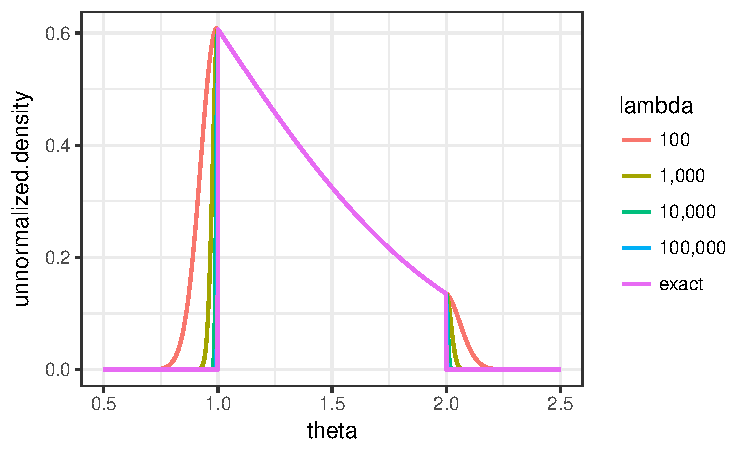
\includegraphics[width=0.5\textwidth]{density_truncated_normal}
\caption{Unnormalized densities for truncated normal $\No_{(1,2)}(0,1)$, under exact and approximating densities. The exact density abruptly drops to $0$ on the two boundaries, while the approximating ones drop continuously. In the approximation, larger $\lambda$ is associated with lower tolerance for constraint violation ($( 1-\theta )_+$ and $( \theta - 2)_+$). All densities inside $(1,2)$ are the same up to a constant difference.}
\label{truncated_normal}
\end{figure}

It is tempting to use very large $\lambda$ for all models. However, when the constrained space $\mc D$ has a geometry not suitable for discrete step update in $\mc R$ (as commonly used in HMC), large $\lambda$ would cause slow posterior mixing. Since the approximation can be eventually corrected in an additional step, it is rather useful to first use a smaller $\lambda$ to induce a larger space expansion for efficient posterior sampling. We will illustrate this via an example in next section.

\subsection{Posterior Sampling for Extrinsic Posterior}

Extrinsic posterior is the approximation to the ones under exact formulation. As it is defined on a less restrictive space $\mc R$, it can be sampled easily. The tradiational sampling tools such as slice sampling, adaptive Metrohepolis-Hastings can be utilized. In this section, we present the sampling algorithm using Hamiltonian Monte Carlo (HMC), due to its high-level automation aided by software and excellent performance in convergence and posterior mixing. Various adaptive algorithms such as \cite{hoffman2014no} have been developed for making the new state less correlated with the current state.

In using the conventional HMC, we assume the space $\mc R$ is an Euchledean space and the constraint functions $E_k(\theta)$'s and $G_k(\theta)$'s  are differentiable with respect to $\theta$. We focus on the case where $\theta$ is continuous, although discrete extension is possible \citep{zhang2012continuous}.

HMC is essentially a data augmentation based MCMC. Using a latent variable named ``veolicty'' $p$ with the same dimension as $\theta$, the negative log-posterior function based on \eqref{extrinsic_prior} is

\begin{equation}
\begin{aligned}
H(\theta, p)& = U(\theta)+M(p),\\
\text{where } & U(\theta) = -\log\left\{ L(\theta;y)\pi_{0,\mc R}(\theta) \mc{E}(\theta) \right\},\\
& M(p) = \frac{p'\Sigma^{-1} p}{2},\end{aligned}
\end{equation}
with $\Sigma^{-1}$ a pre-specified positive definite matrix. Unlike conventional MCMC, HMC utilizes the Hamiltonian dynamics based on the solution to the differential equations:

\begin{equation}
\begin{aligned}
\label{hamiltonian}
\frac{\partial \theta (t)}{\partial t} & =\frac{\partial H(\theta, p)}{\partial p} = \Sigma^{-1}p,\\
\frac{\partial p(t)}{\partial t}& =-\frac{\partial H(\theta, p)}{\partial \theta} = -\frac{\partial U(\theta)}{\partial \theta}.
\end{aligned}
\end{equation}

At each step, the current state of $\theta$ is viewed as $\theta(0)$ with $p(0)$ randomly generated from $\No(0, \Sigma)$. Then they enter the Hamiltonian dynamics to generate $\theta(t)$ and $p(t)$. An Metropolis-Hastings step is taken at the end to accept $\theta(t)$ with probability $1\wedge \exp  \left( - H(\theta(t),p(t)) + H(\theta(0),p(0))\right)$. When solution to \eqref{hamiltonian} has closed-form, the acceptance rate is always $1$. However, often numerical approximation with discrete movement is commonly needed, such as the leap-frog algorithm \citep{neal2011mcmc}:

\begin{equation}
\begin{aligned}
\label{leap-frog}
p(T+ \epsilon/2) & = p(T) - \epsilon/2 \frac{\partial U}{\partial  \theta } ( \theta (T)),\\
 \theta (T + \epsilon) & =  \theta (T) + \epsilon \Sigma^{-1}p(T+  \epsilon/2),\\
p(T+ \epsilon) &= p(T+ \epsilon/2) - \epsilon/2 \frac{\partial U}{\partial  \theta } ( \theta (T + \epsilon)),
\end{aligned}
\end{equation}
for $T=0,\epsilon, 2\epsilon,\ldots, L\epsilon$, with $L$ as the total steps within one iteration and $t= L\epsilon$.

Due to the cost of multiple steps, one would hope to utilize relatively large $\epsilon$ with relatively small $L$. This could bring some further implication on choosing $\lambda$ in the extrinsic prior $\mc E(\theta)$. Specifically, one needs to ensure a decent-sized discrete move along $\frac{\partial U(\theta)}{\partial \theta}$ does not end in a low posterior density region; otherwise, only a small step size $\epsilon$ can be used.

For example, when $\mc D$ is a truncated Euchledean space defined by simple space truncation, random move along certain directions of $\frac{\partial U(\theta)}{\partial \theta}$ can still lead to high posterior region its internal space of $\mc D$, therefore large $\lambda$ generally do not impact the effectiveness of using large $\lambda$. On the other hand, when $\mc D$ is on a unit circle, random move along any Euchledean direction will move away from this space. With very large $\lambda$, the high posterior density region would be very narrow, demanding a small $\epsilon$. In this case, a smaller $\lambda$ inducing a greater support expansion would be more useful, since it allows more efficient Hamiltonian dynamics.
 
To illustrate the latter case, consider generating a random variable $\theta=(x_1,x_2)$ on a unit circle using von Mises--Fisher distribution, $\pi(\theta \mid y) \propto \exp(F'\theta)$ with $\theta'\theta =1$. This is a simple example of a random variable constraint on a $(2,1)$-Stiefel manifold $\mc D =\mc V(2,1)$. We set $F=(1,1)$ to induce a distribution widely spreaded over the manifold, generating great amount of uncertainty to assess the mixing performance. We use extrinsic prior proportional to $K(\theta)= \exp(-\lambda (\theta'\theta -1)^2) \mathbbm{1}_{|\theta'\theta -1|<0.1}$. Geometrically, the extrinsic prior expands the posterior support from a circle to a ring, with its radius defined by the maximally tolerable constraint violation. 

\begin{figure}[H]
 \centering
    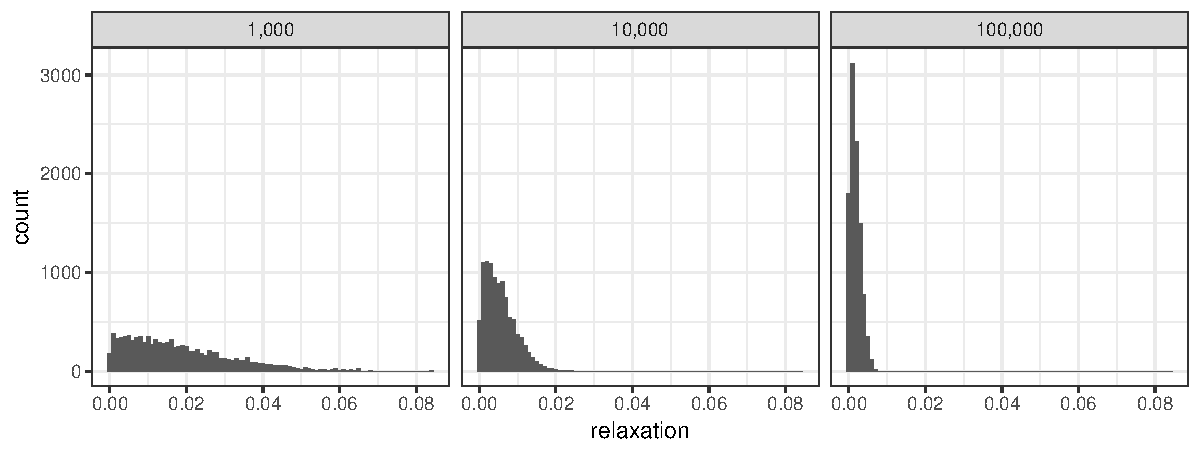
\includegraphics[width=0.8\textwidth]{unit_circle_violation}
  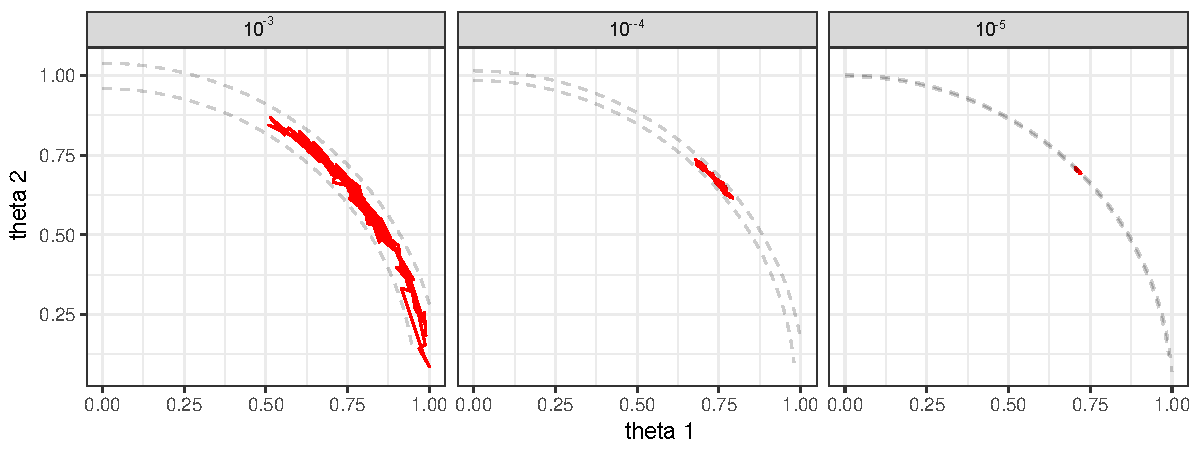
\includegraphics[width=0.8\textwidth]{unit_circle_100steps}
 % 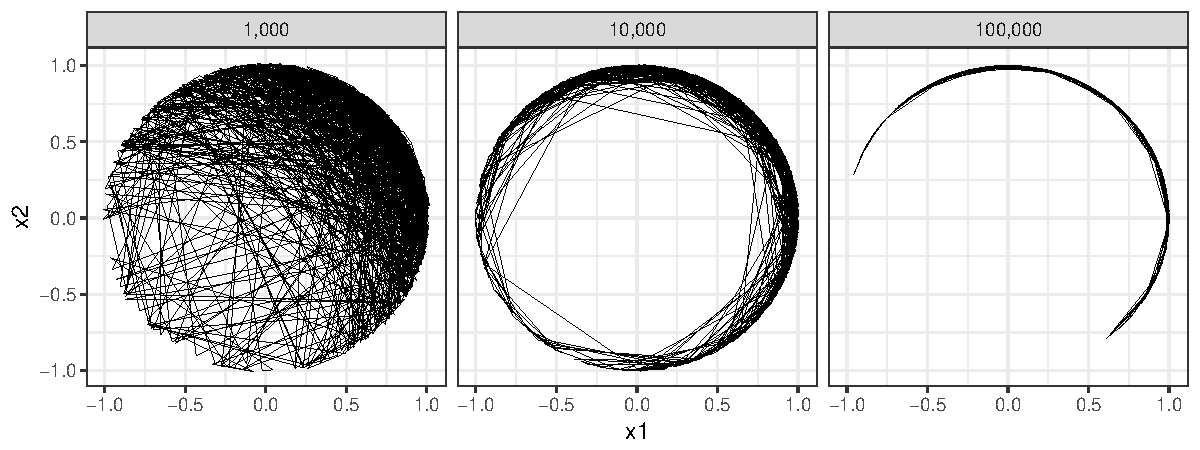
\includegraphics[width=0.8\textwidth]{unit_circle_path}
 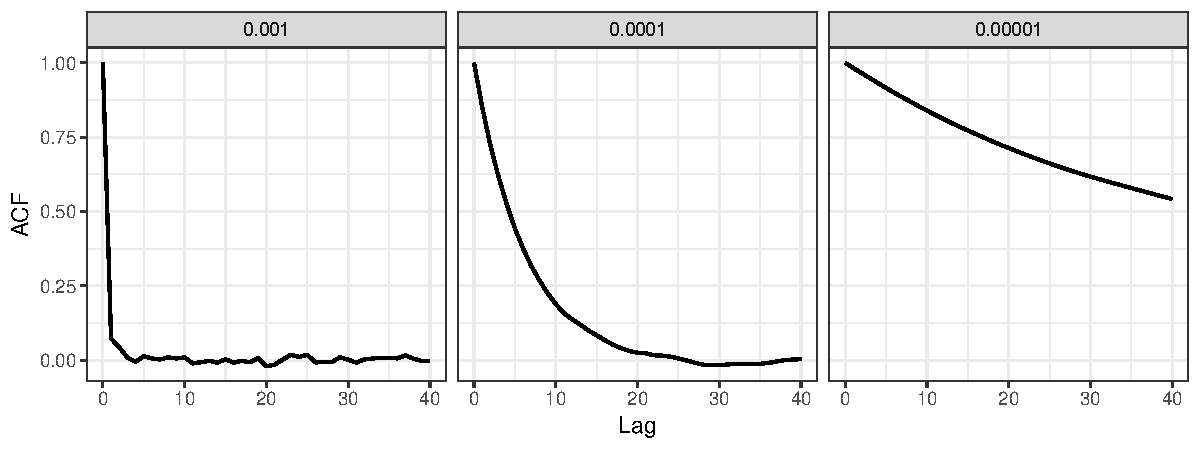
\includegraphics[width=0.8\textwidth]{unit_circle_acf}
\caption{Sampling posterior from a von Mises--Fisher distribution on a unit circle, using HMC with extrinc prior under $\lambda=10^3,10^4,10^5$. Row $1$ shows the posterior distribution of the constraint violation $|\theta'\theta -1|$; Row $2$ shows the path of $1,000$ leap-frog steps; Row $3$ shows the autocorrelation plot (ACF). Large $\lambda$ results in small constraint violation, but suffers from slow mixing due to inefficient local update; smaller $\lambda$ increases the approximation error but results in excellent mixing.}
\label{unit_circle}
\end{figure}


We tested three different values of $\lambda = 10^3,10^4,10^5$  associated with different radii. For each $\lambda$, we ran HMC for $10,000$ iterations, with $L=100$ leap-frog steps in each iteration. 
We use $\Sigma= \diag(1,1)$ to generate velocity. During the initial $2,000$ iterations, the leap-frog step size $\epsilon$ is automatically tuned for an acceptance rate close to $0.6$, then it is fixed during the remaining part of Markov chain. The last $5,000$ iterations are used as posterior samples. Figure~\ref{unit_circle} plots the posterior distribution of constraint violation $|\theta'\theta -1|$, the sampling path and the autocorrelation function (ACF) for each Markov chain. Very large $\lambda=10^5$ has much less constraint violation; however, due to the narrow radius of the ring, the associated HMC has small $\epsilon$ and can only explore local space for each $100$ steps. This results in a very slow mixing (large autocorrelation even at 40 lags). On the other hand, smaller $\lambda=10^3$ has slightly larger constraint violation, but allows much more efficient exploration of the space and excellent mixing performance.




\subsection{Correcting Projection to Constraint Space}
 
The Markov chain produced by HMC is geometrically ergodic under very general conditions \citep{livingstone2016geometric}. With the extrinsic posterior $\pi_K(\theta \mid y)$ as approximation to \eqref{exact_posterior}, one may be interested in further obtaining exact posterior in $\mc D$, likely for two reasons:  (1) to strictly uphold the constraints; (2) to erase the loose error control during extrisinc posterior sampling.

Letting $\theta^*$ be a random sample collected based on $\pi_K(\theta \mid y)$, there exists deterministic projection $M: \mc R\rightarrow \mc D$ and obtain $\theta^*_{\mc D}= M(\theta^*)$. Using this as proposal machineary, one can construct another Markov chain based on $\pi(\theta_{\mc D}  \mid y)$. Letting the current state be $\theta_{\mc D} = M(\theta)$, we generate proposal $\theta^*_{\mc D}= M(\theta^*)$ and accept it with probability:

\begin{equation}
 \begin{aligned}
 1 \wedge \frac{\pi(\theta^*_{\mc D} \mid y) \pi_K(\theta  \mid y) }{\pi(\theta_{\mc D}  \mid y)\pi_K(\theta^* \mid y)} =  1 \wedge \frac{\ L(\theta^*_{\mc D};y)\pi_{0,\mc R}(\theta^*_{\mc D})  \cdot    L(\theta;y)\pi_{0,\mc R}(\theta)   \mc E(\theta)}{\ L(\theta_{\mc D};y)\pi_{0,\mc R}(\theta_{\mc D})   \cdot L(\theta^*;y)\pi_{0,\mc R}(\theta^*)   \mc E(\theta^{*})}.
 \end{aligned}
 \end{equation}
 
The remaining task is then to optimize the projection with respect to the acceptance rate. Noting 

\begin{equation}
\begin{aligned}
% |\log( \frac{\pi(\theta^*_{\mc D} \mid y) \pi_K(\theta  \mid y) }{\pi(\theta_{\mc D}  \mid y)\pi_K(\theta^* \mid y)}) | \ge \big| |\log( \pi(\theta^*_{\mc D} \mid y)) - \log( \pi_K(\theta^* \mid y))| - |\log( \pi(\theta_{\mc D} \mid y)) - \log( \pi_K(\theta \mid y))| \big| \\
|\log( \frac{\pi(\theta^*_{\mc D} \mid y) \pi_K(\theta  \mid y) }{\pi(\theta_{\mc D}  \mid y)\pi_K(\theta^* \mid y)}) | \le |\log \left( \pi(\theta^*_{\mc D} \mid y) \right) - \log \left( \pi_K(\theta^* \mid y) \right)| + |\log \left( \pi(\theta_{\mc D} \mid y)\right) - \log\left( \pi_K(\theta \mid y)\right)|,
\end{aligned}
\end{equation}
it is sensible choose $\theta_{\mc D}=M(\theta)$ to minimize the difference $Q(\theta_{\mc D})=\left|\log( \pi(\theta_{\mc D} \mid y)) - \log( \pi_K(\theta \mid y))\right| = \left|\log L(\theta_{\mc D};y)\pi_{0,\mc R}(\theta_{\mc D}) - \log L(\theta;y)\pi_{0,\mc R}(\theta)   \mc E(\theta) \right|$ towards $0$ for each sample in the extrinsic posterior. Obviously, when the approximate $\theta \in \mc D$ exactly, the optimal projection would be the identity function; when $\theta \not\in \mc D$, standard optimization technique can be used.

Continuing the unit circle example, we first obtain $\hat\theta_{\mc D} =  \underset{\theta_{\mc D}:\theta_{\mc D}'\theta_{\mc D}=1 }{\text{argmin}}|  F'\theta_{\mc D}  - \{ F'\theta  - \lambda (\theta'\theta -1)^2 \}|$ based on the extrinsic posterior sample collected with $\lambda =10^3$. Then we construct the exact Markov chain and obtained acceptance rate $96.9\%$.

\subsection{Specification of Hyper-parameter}

\leo{Need some formalization here:}.

Two possible ways to formalize the choice for hyper-parameter $\lambda$:

1. Compute some similarity measure between the local behavior of the constrained space $\mc D$ and the embedded space $\mc R$. Parameterize $\lambda$ as the function of this similarity. When similarity is low, use smaller $\lambda$ to expand the posterior support.

2. Use something similar to the compminimax idea. First use minimum acceptance rate to derive a maximally tolerable violation, then optimize the mixing rate. 


\section{Illustration}

{\bf Example 1: Ordered Simplex}

{\bf Example 2: Monotone Spline} 

{\bf Example 3: Orthonormal Gaussian Processes} 

\section{Theory}

Posterior properiety of $\pi_{0,\mc R}(\theta) \mc E(\theta)$,  when $\pi_{0,\mc D}(\theta)$ is proper but $\pi_{0,\mc R}(\theta)$ is improper. 

\section{Application}
\section{Discussion}



\bibliography{reference}
\bibliographystyle{chicago}

\end{document}
